\documentclass[8pt]{beamer}
\mode<presentation>
{
  \usetheme{Madrid}
  \usefonttheme{default}
}
\renewcommand{\baselinestretch}{1.5}
%\usepackage[legalpaper, landscape, margin=2in]{geometry}
\usepackage[utf8]{inputenc}
\usepackage[T1]{fontenc}
\usepackage{graphicx}
\usepackage{tikz}
\usepackage{circuitikz}
\usepackage{hyperref}
\usepackage{listings}
\usepackage{multicol}
\setlength{\columnsep}{4.5cm}

\title[Report]{A Fourier Perspective on Model Robustness in Computer Vision}
\author{Krishna Srikar Durbha}
\date{21st October 2020}

\begin{document}

\begin{frame}
  \titlepage
\end{frame}

\begin{frame}
\frametitle{Table of Contents}
\tableofcontents
\end{frame}

\section{Introduction}
\begin{frame}[allowframebreaks]{Problem with Distributional Shift}
\textbf{Distributional Shift:}\\
\qquad If Train and Test sets are not from the same Distribution such a shift is called Distributional Shift. Covariate Shift may be the most widely studied. We assume that while the distribution of inputs may change over time, the labeling function, i.e., the conditional distribution $P(y|\textbf{x})$  does not change. Statisticians call this Covariate shift because the problem arises due to a shift in the distribution of the Covariates (features).

\vspace{0.25in}

\textbf{Example:}\\
\qquad If Model is trained on Images from Fig.\ref{fig:Train Images} and when test on Images from Fig.\ref{fig:Test Images}. There is a substantially difference in characteristics between the Train and Test Set as Training Set contains Real-World Images while Test set contains Cartoons.

\framebreak

\begin{figure}
    \centering
    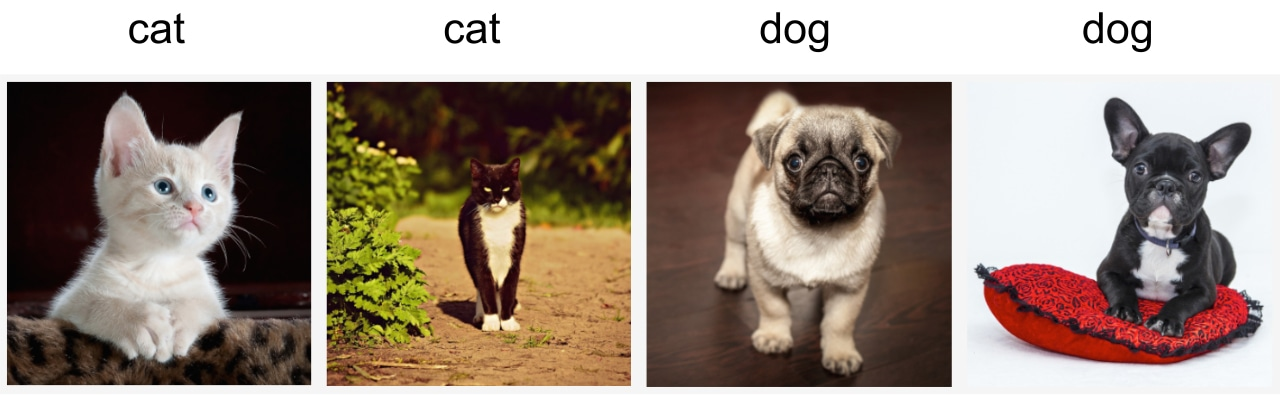
\includegraphics[scale=0.2]{../Images/cat-dog-train.jpg}
    \caption{Train Images}
    \label{fig:Train Images}
\end{figure}

\begin{figure}
    \centering
    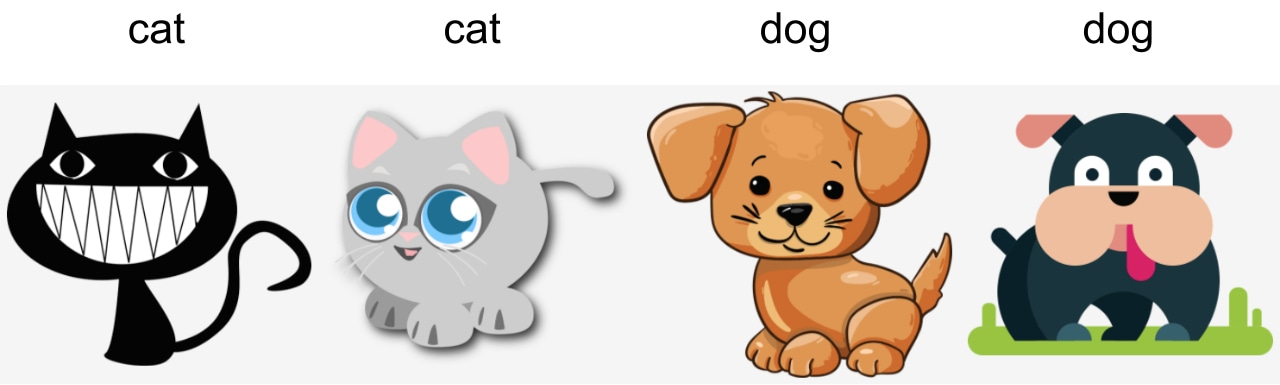
\includegraphics[scale=0.2]{../Images/cat-dog-test.jpg}
    \caption{Test Images}
    \label{fig:Test Images}
\end{figure}
\end{frame}

\section{Data Augmentation}
\begin{frame}{Data Augmentation}
\textbf{Data Augmentation:}\\
\qquad Data Augmentation is the process of increasing the amount and diversity of data. We do not collect new data, rather we transform the already present data. Data Augmentation is a natural and sometimes effective approach to learning robust models.\\ \qquad Examples of data augmentation include Adversarial Training, applying Image Transformations to the training data, such as flipping, cropping, adding Random Noise, and even stylized image transformation.
\end{frame}

\section{Gaussian Data Augmentation and Adversarial Training}
\begin{frame}[allowframebreaks]{Gaussian Data Augmentation and Adversarial Training}
\textbf{Gaussian Data Augmentation:}\\
\qquad Gaussian Data Augmentation Technique integrates Signal-to-Noise Ratio (SNR) with an Additive White Gaussian Noise (AWGN) to generate derived data samples suited for multi-class classification in various Deep Neural Networks Models. 

\vspace{0.2in}

\textbf{Adversarial Training:}\\
\qquad The process of training the model on adversarially perturbed examples from the training set in the context of Regularization i.e inorder to reduce error on Test set. Adversarial training discourages this highly sensitive locally linear behavior by encouraging the network to be locally constant in the neighborhood of the training data. This can be seen as a way of explicitly introducing a local constancy prior into supervised neural nets.

\framebreak

\textbf{Examples of Adversarial Example Generation:}\\
\begin{figure}
    \centering
    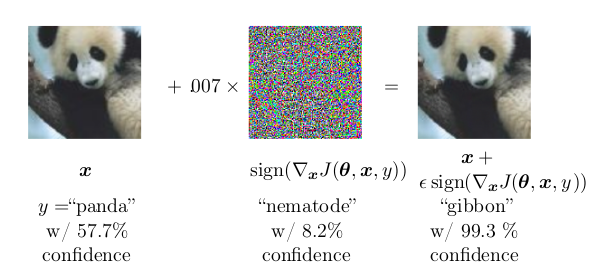
\includegraphics[scale=0.4]{../Images/Adversarial Training.png}
    \caption{A demonstration of adversarial example generation applied to GoogLeNet on ImageNet. By adding an imperceptibly small vector whose elements are equal to the sign of the elements of the gradient of the cost function with respect to the input, we can change GoogLeNet’s classification of the Image. (Source: \href{https://www.deeplearningbook.org/}{Deep Learning Book})}
    \label{fig:my_label}
\end{figure}
\end{frame}

\section{2D-Gaussian Distribution}
\begin{frame}[allowframebreaks]{2D-Gaussian Distribution}
\begin{figure}[ht]
    \begin{minipage}[b]{0.45\textwidth}
        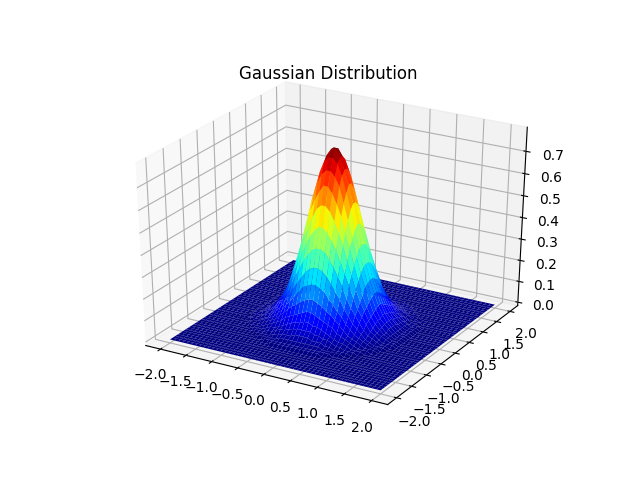
\includegraphics[scale=0.35]{../Images/Gaussian.png}
        \caption{2D-Gaussian Distribution}
        \label{fig:GD}
    \end{minipage}
    \begin{minipage}[b]{0.45\textwidth}
        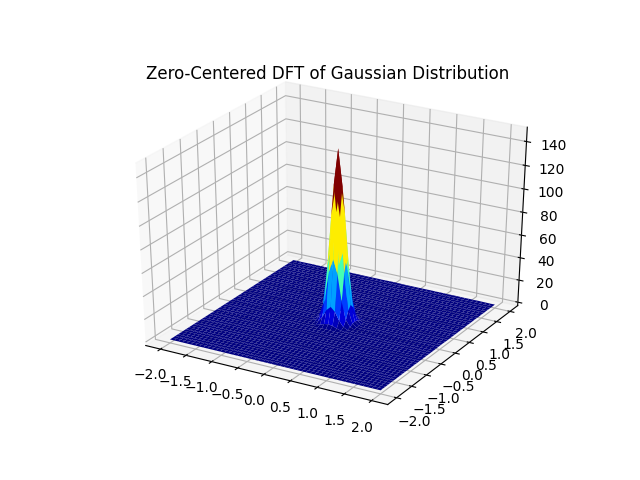
\includegraphics[scale=0.35]{../Images/ZeroCentered_Gaussian_DFT.png}
        \caption{DFT of 2D-Gaussian Distribution}
        \label{fig:DGD}
    \end{minipage}
\end{figure}
\framebreak
\begin{figure}[ht]
    \begin{minipage}[b]{0.45\textwidth}
        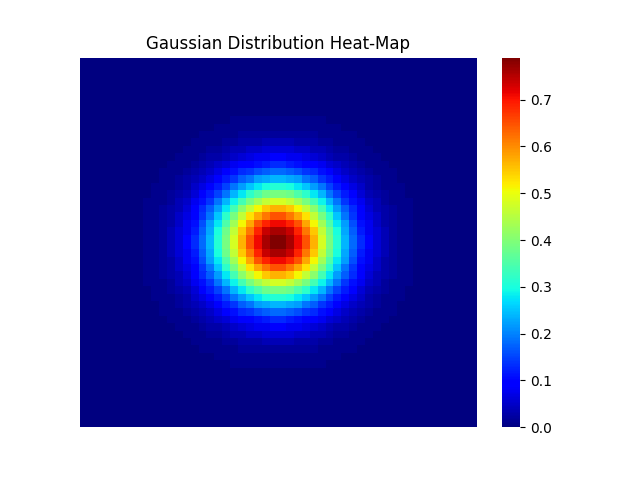
\includegraphics[scale=0.35]{../Images/Gaussian_HeatMap.png}
        \caption{Heat-Map of 2D-Gaussian}
        \label{fig:GDH}
    \end{minipage}
    \begin{minipage}[b]{0.45\textwidth}
        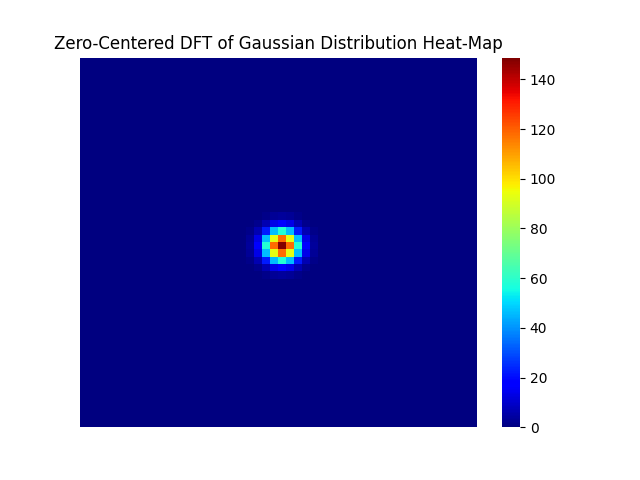
\includegraphics[scale=0.35]{../Images/ZeroCentered_Gaussian_DFT_HeatMap.png}
        \caption{Heat-Map of DFT of 2D-Gaussian}
        \label{fig:DGDH}
    \end{minipage}
\end{figure}
\end{frame}

\section{Hypothesis and Solution}
\begin{frame}{Hypothesis and Solution}
\textbf{Hypothesis:}\\
\qquad Operating Hypothesis of the paper is that the frequency information of these different corruptions offers an explanation of many of these observed trade-offs. Through extensive experiments involving perturbations in the Fourier domain, it is demonstrated that Augmentation Procedures like Gaussian Data Augmentation and Adversarial Training bias the model towards utilizing \textbf{Low Frequency Information} in the Input. This Low Frequency Bias is making the Model robust on High Frequency Corruptions (Corruptions primarily effecting High Frequency Content) while they are degrading performance on Low Frequency Corruptions.\\
\vspace{0.2in}
\textbf{Solution:}\\
\qquad More diverse Data Augmentation Procedures could be leveraged to mitigate the trade-offs called \textbf{AutoAugment}. \textbf{AutoAugment} Data Augmentation achieves state-of-the art results on the CIFAR-10-C benchmark and ImageNet-C
\end{frame}

\section{Perturbations and Investigation}
\begin{frame}{Perturbations and Investigation}
\qquad A parameter $\sigma$ for the following operation: In each iteration, we add i.i.d. Gaussian Noise $\mathcal{N}(0,\tilde{\sigma}^2)$ to every pixel in all the images in the training batch, where $\tilde{\sigma}$ is chosen uniformly at random from $[0, \sigma]$.  When Gaussian Data Augmentation is used, $\sigma = 0.1$ for CIFAR-10 and $\sigma = 0.4$ for ImageNet.\\
\vspace{0.1in}
\textbf{Sensitivity of Models:}\\
In-order to investigate sensitivity of models towards corruptions, we define a $U_{i,j} \in \mathbb{R}^{d_1 \times d_2}$ called 2D-Fourier Basis Matrices which have the following properties:\\
\begin{enumerate}
    \item $||U_{i,j}|| = 1$
    \item $\mathcal{F}(U_{i,j})$ only has up to two non-zero elements located at (i, j) and the its symmetric coordinate with respect to the image center.
\end{enumerate}

We perturbed Images with Fourier basis noise. $\tilde{X}_{i,j} = X + rvU_{i,j}$, where r is chosen uniformly at random from $\{-1, 1\}$, and v > 0 is the norm of the perturbation. Models are evaluated under Fourier Basis Noise and visualization are made how the test error changes as a function of (i, j), and these results are called Fourier Heat Map of a Model.
\end{frame}

\section{Understanding Robustness Problem}
\begin{frame}[allowframebreaks]{Understanding Robustness Problem}
\qquad In an Images, there are a lot of Correlations between the Input and Target that Models can utilize to Generalize. If Model uses such Statistics, as they can be corrupted, this will lead to dramatic decrease in performance of Model.\\
\vspace{0.05in}
\qquad Simple Statistics such as Colors, Local Textures, Shapes, even un-intuitive High frequency Patterns can all be leveraged in a way to achieve remarkable i.i.d generalization. If Models use these features for generalisation, Model are not-robust as these features can be corrupted easily.\\
\vspace{0.05in}
\qquad A Natural Assumption is that Data Augmentation may bias the model towards utilizing different kinds of features during classification. But the truth is Features used by the Model ultimately determine its Robustness during Test time.\\
\vspace{0.05in}
\textbf{Demonstration:} Models can achieve high accuracy using information from the input that would be unrecognizable to humans. Models trained and tested with aggressive high and low pass filtering applied to the inputs. High Pass filtered images needed be normalized to have unit variance in order to properly visualize the high frequency features.
\framebreak
\begin{figure}
    \centering
    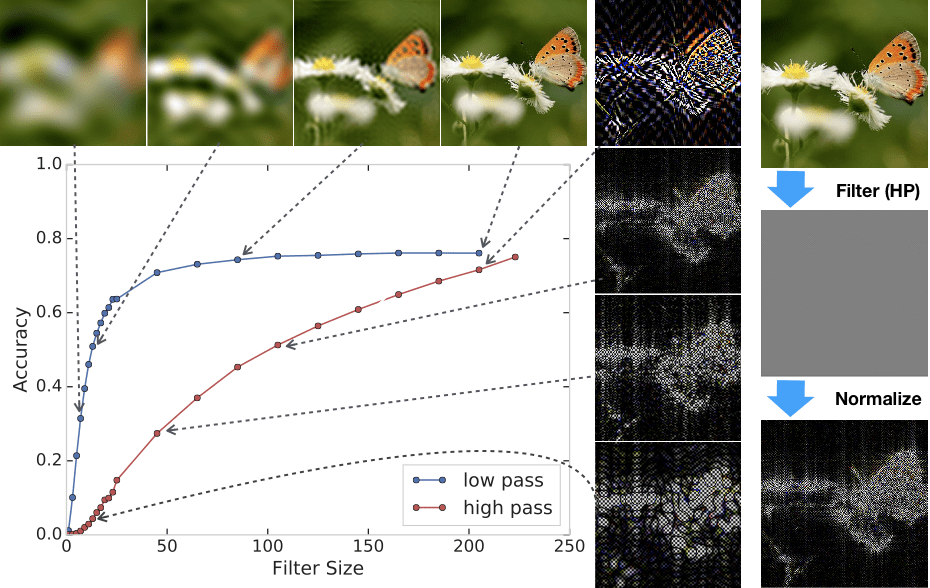
\includegraphics[scale=0.25]{../Images/Robustness.png}
    \caption{With aggressive Low-Pass Filtering, the Model is still above 30\% on ImageNet when the images appear to be simple globs of color. In the case of high-pass (HP) filtering, models can achieve above 50\% accuracy using features in the input that are nearly invisible to humans.}
    \label{fig:Robustness}
\end{figure}
\end{frame}

\section{Trade-off and Correlation between Corruptions: A Fourier Perspective}
\begin{frame}[allowframebreaks]{Gaussian data Augmentation and Adversarial Training Bias Models towards Low Frequency information}
\qquad When 3 Models, Naturally trained, by Gaussian Data Augmentation and Adversarially trained are trained on CIFAR-10-C dataset, it is observed that both Gaussian Data Augmentation and Adversarial Training are increasing Model Robustness where as degrading performance to fog and contrast.\\

\textbf{Corruptions:}
Assuming a Corruption Function by $\mathcal{C}:\mathbb{R}^{d_1 \times d_2} \to \mathbb{R}^{d_1 \times d_2}$,
\begin{enumerate}
    \item For Blurring Corruption, generally High Frequency Components are modified. So, $\mathcal{C}(X) - X$ will have High Frequency Energy.
    \item Corruptions such as Contrast and Fog, energy of the corruption is concentrated more on Low Frequency Components.
\end{enumerate}
\framebreak
\begin{figure}
    \centering
    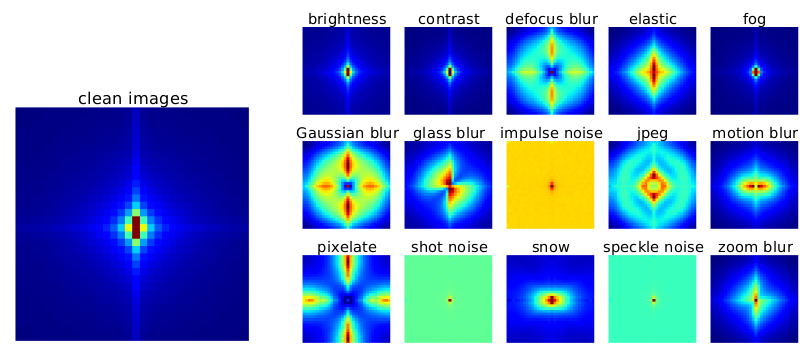
\includegraphics[scale=0.35]{../Images/Augmentation.png}
    \caption{Left: Fourier spectrum of natural images; we estimate $E[|\mathcal{F}(X)[i, j]|]$ by averaging all the CIFAR-10 validation images. Right: Fourier spectrum of the corruptions in CIFAR-10-C. For each corruption, we estimate $E[|\mathcal{F}(\mathcal{C}(X) - X)[i, j]|]$ by averaging over all the validation images.}
\end{figure}
\end{frame}

\section{Observations}
\begin{frame}{Observations}
\textbf{Observations:}\\
\qquad The naturally trained model is highly sensitive to additive perturbations in all but the lowest frequencies, while Gaussian Data Augmentation and Adversarial Training both dramatically improve Robustness in the Higher Frequencies. For the models trained with Data Augmentation, there is a lack of robustness at the lowest frequencies (relative to the naturally trained model).\\
\vspace{0.1in}
\qquad Performance of Models is further verified by applying low/high pass filter (we call the low/high pass filters the front end of the model) to the input. The results are when we apply a low-pass front-end it degrades Performance of model on Fog and Contrast while Improving Performance on Additive Noise and Blurring.\\
\vspace{0.05in}
\qquad If we try to Bias the Model towards High Frequency Information, performance on all corruptions is effected and performance degradation is severe for high frequency corruptions.
\end{frame}

\section{Results}
\begin{frame}[allowframebreaks]{Results}
\begin{figure}
    \centering
    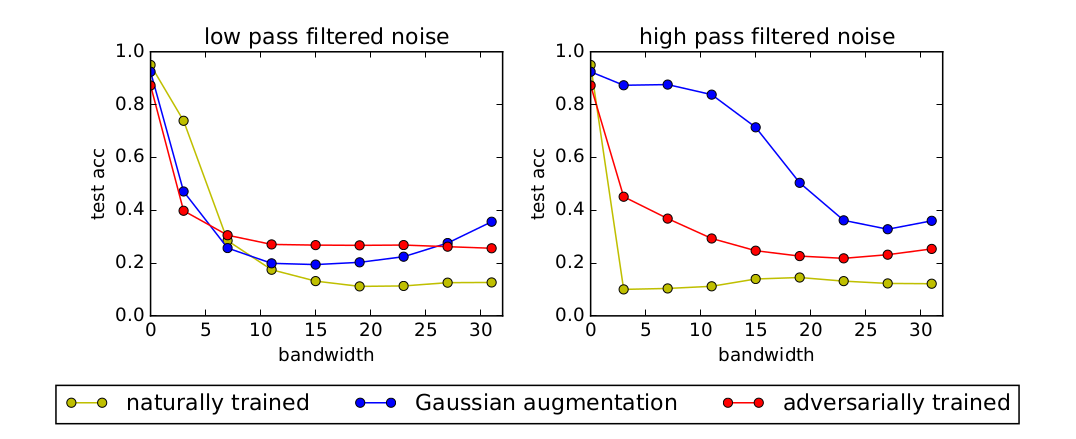
\includegraphics[scale=0.3]{../Images/Observations.png}
\end{figure}\\

\framebreak

\textbf{Results:}\\
Robustness of models under additive noise with fixed norm and different frequency distribution. We vary the bandwidth of the low/high pass filter and generate the two plots. The naturally trained model is more robust to the low frequency noise with bandwidth 3, while Gaussian data augmentation and adversarial training make the model more robust to high frequency noise.\\
\vspace{0.1in}
\qquad Low Frequency Data Augmentation similar to Fog Corruption also doesn't help. It also degrades performance of Model on Fog Corruption although resulting model is robust to perturbations along with Low Frequency Vectors. So, we can assume that Low Frequency are more complicated that High Frequency Corruptions as Natural Images are more concentrated more in low frequencies information, the model can learn to ignore high frequency information. It can also been observed that, Model Performance degrades rapidly when low frequency information is removed than high frequency.\\

\end{frame}

\section{AutoAugment}
\begin{frame}[allowframebreaks]{AutoAugment}
\qqaud AutoAugment applies a learned Mixture of Image Transformations during Training and Achieves the state-of-the-art Performance.

\begin{figure}
    \centering
    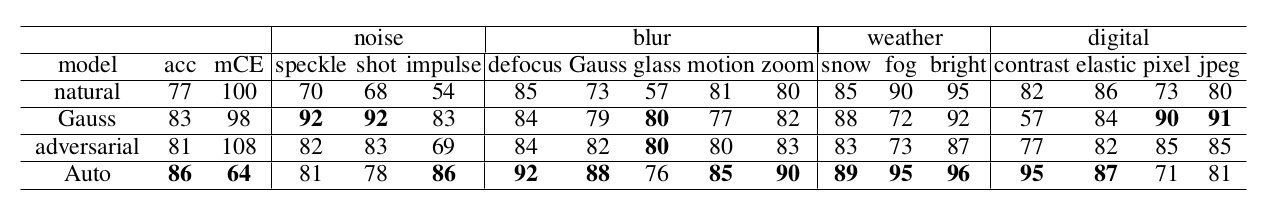
\includegraphics[scale=0.25]{../Images/Results.png}
    \caption{Comparisons between Naturally Trained Model (natural), Gaussian Data Augmentation (Gauss), Adversarially Trained Model (adversarial), and AutoAugment (Auto) on CIFAR-10-C.}
\end{figure}

\framebreak

\begin{figure}
    \centering
    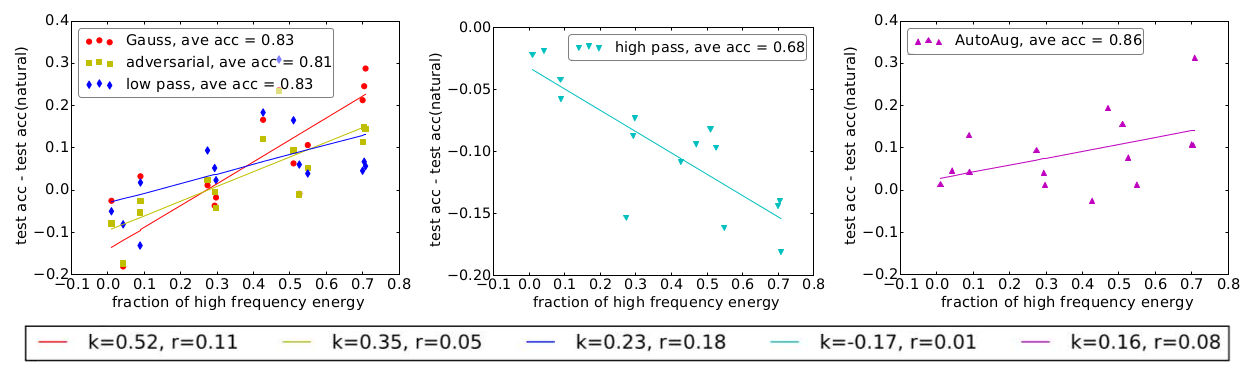
\includegraphics[scale=0.25]{../Images/FrequencyResults.png}
    \caption{Relationship between test accuracy and fraction of high frequency energy of the CIFAR-10-C corruptions. The x-axis represents the fraction of high frequency energy of the corruption type, and the y-axis represents change in test accuracy compared to a naturally trained model. Overall, Gaussian data augmentation, adversarial training, and adding low pass filter improve robustness to high frequency corruptions, and degrade robustness to low frequency corruptions. Applying a high pass filter front end yields a more significant accuracy drop on high frequency corruptions compared to low frequency corruptions. AutoAugment improves robustness on nearly all corruptions, and achieves the best overall performance.}
\end{figure}
\end{frame}

\section{Fourier Perspective on Adversarial Examples}
\begin{frame}[allowframebreaks]{Fourier Perspective on Adversarial Examples}
\qqaud A common hypothesis is that Adversarial Perturbations lie primarily in the High Frequency Domain. Adversarial examples are not strictly a High Frequency Phenomenon. Studying the statistics of adversarially generated perturbations is not a well defined problem because these statistics will ultimately depend on how the adversary constructs the perturbation.\\
\vspace{0.1in}
\textbf{Procedure:}\\
\qqaud We then analyze the delta between the clean and perturbed images and project these deltas into the
Fourier domain. By aggregating across the successful attack images, we obtain an understanding of the frequency properties of the constructed adversarial perturbations. For the Naturally Trained Model, the measured adversarial perturbations do indeed show higher concentrations in the high frequency domain relative to the statistics of natural images. But Adversarial Training encourages these perturbations to be more concentrated in Low Frequency Domain.\\

\framebreak

\begin{figure}
    \centering
    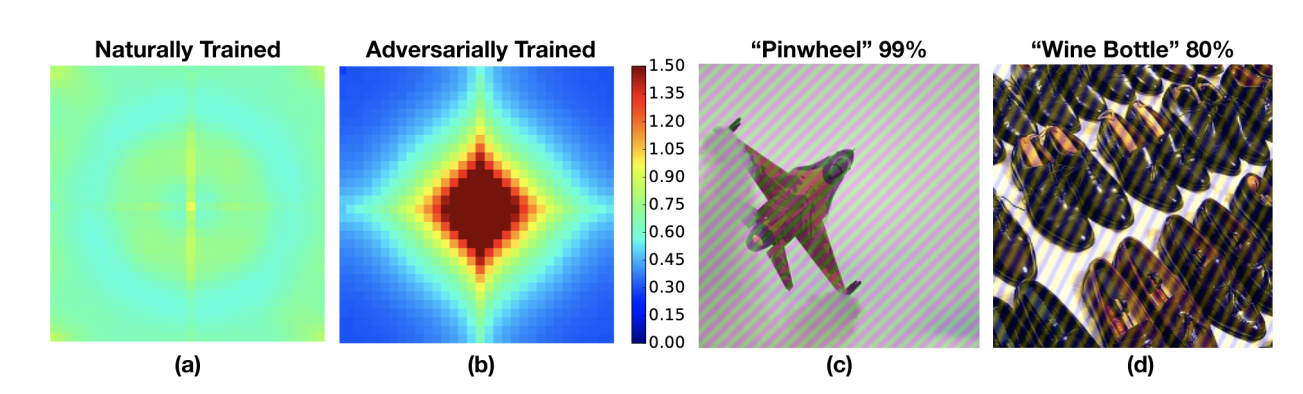
\includegraphics[scale=0.25]{../Images/AdversarialFourier.png}
    \caption{(a) and (b): Fourier spectrum of adversarial perturbations. For any image X, we run the PGD (Projected Gradient Descent) attack to generate an adversarial example $\mathrm{C}(X)$. We estimate the Fourier spectrum of the adversarial perturbation, i.e., E[|F(C(X) − X)[i, j]|], where the expectation is taken over the perturbed images which are incorrectly classified. (a) naturally trained; (b) adversarially trained. The adversarial perturbations for the naturally trained model are uniformly distributed across frequency components. In comparison, adversarial training biases these perturbations towards the lower frequencies. (c) and (d): Adding Fourier basis vectors with large norm to images is a simple method for generating content-preserving black box adversarial examples.}
\end{figure}
\end{frame}

\section{Conclusion}
\begin{frame}{Conclusion}
\begin{enumerate}
    \item Gaussian Data Augmentation and Adversarial Training bias the model towards low frequency information in the input.
    \item Impressive Robustness is observed by using AutoAugment. This gives us hope that Data Augmentation done properly can play a crucial role in mitigating the Robustness Problem.
    \item Data Augmentation must to done carefully to avoid Over-fitting as the goal is to learn \textbf{Domain Invariant Features}
    \item The robustness problem is certainly far from solved, and our Fourier analysis shows that the AutoAugment model is not strictly more robust than the baseline — there are frequencies for which robustness is degraded rather than improved.
\end{enumerate}
\end{frame}
\end{document}
